\section{Introduction}
\label{sec:introduction}

% % Underwater Robot Applications:
%
Operating in complex, hazardous, and otherwise inaccessible environments, \Acfp{ROV} have become essential for a diverse range of demanding applications, including surveying, infrastructure inspection, and search-and-rescue, significantly expanding operational possibilities~\cite{amer2023unav, amer2025modelling}.
%
% Why We Need Tether:
%
Most \acp{ROV} are tethered to ensure a continuous power supply during long-duration missions and to maintain reliable communication.
%
% Introducing Problem Definition:
%
However, the presence of a tether introduces complexities in path planning and control, as it poses a risk of entanglement with underwater objects such as flora, fauna, or the underwater structures being inspected.

This challenge restricts the applicability of many path planning algorithms originally designed for untethered drones and surface vehicles. For instance, numerous \ac{CPP} algorithms exist to compute distance-optimal paths for covering 3D structures \cite{bircher2015structural,feng2024fc, amer2023visual}. Additionally, exploration path planners are employed to determine the next viewpoints for mapping and exploring unknown terrains \cite{dang2020graph}. However, these methods do not account for entanglement with the surroundings and thus cannot be directly applied to tethered underwater robots.
%
% Entanglement Problem and Definition:
%
Entanglement occurs when the movement of the underwater vehicle is restricted due to physical interactions between the tether and objects in the environment. Tether can bend or loop around obstacles, limiting vehicle mobility. This work bridges a critical gap in automatic asset inspection by proposing \ac{REACT}.

The contributions of this work can be summarized as follows:
\begin{itemize}
\item A fast online tether model that computes the tether configuration in real time using \ac{SDF} data of arbitrary underwater structures.
\item An efficient online replanning method that prevents entanglement by incorporating a tether length constraint.
\item Integration of the proposed method into a \ac{CPP} framework with \ac{MPC} to enable optimal inspection of underwater structures while avoiding entanglement.

\item Demonstration of the framework in simulation, showcasing its ability to ensure safe and time-efficient inspection.
\end{itemize}


%
\begin{figure}[t!]
	\centering	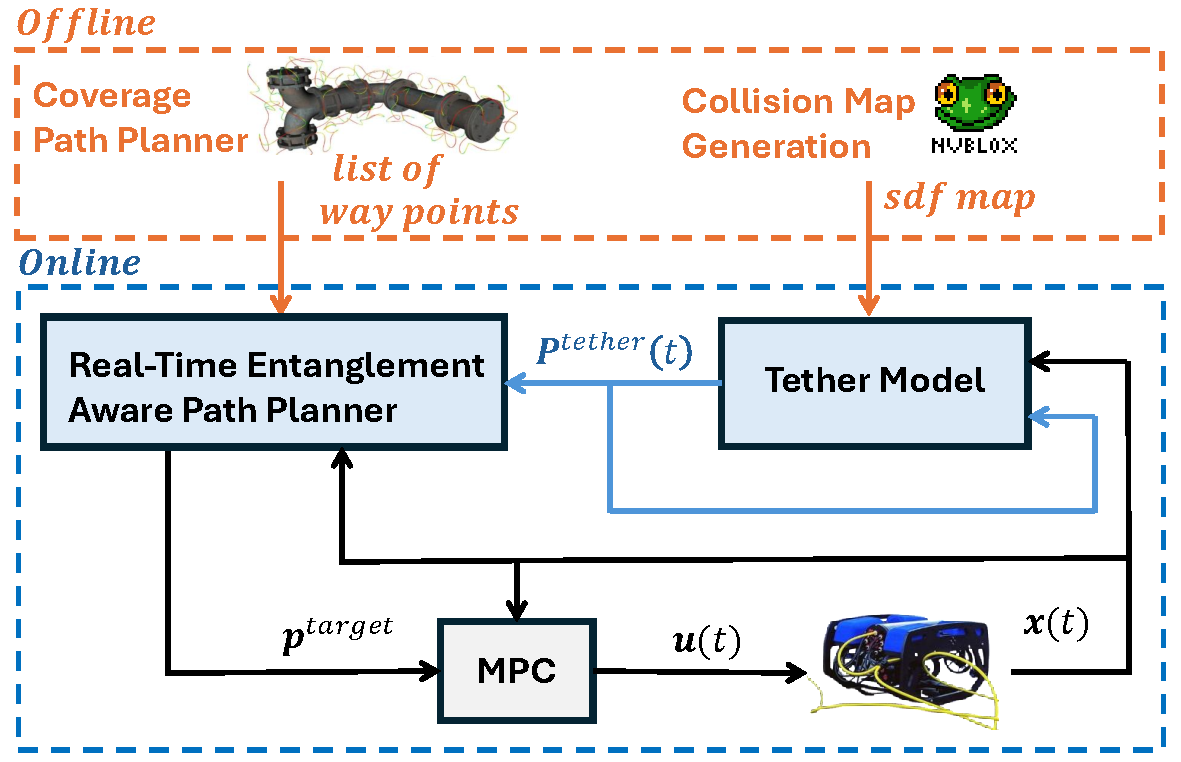
\includegraphics[width=1\linewidth]{EA-Planner/figures/react_abstract.pdf}
	  \caption{\textcolor{black}{Overview of the \ac{REACT} inspection framework. In the offline phase, a \ac{SDF} map is generated from a point cloud, and the FC-Planner \cite{feng2024fc} computes an optimal waypoint sequence. In the online phase, a tether model $\mathbf{P}^{tether}(t)$ ensures the maximum tether length is maintained, while an \ac{MPC} controller applies the optimal wrench $\mathbf{u}(t)$ to the \ac{ROV}}.}
    \label{fig:abstract}
\end{figure}
%







The remainder of this paper is organized as follows: Section \ref{sec:related_work} reviews the state of the art. Section \ref{sec:framework} presents the path planning framework for underwater structure inspection with tether constraints. Section \ref{sec:tether_model} introduces the taut-tether model, and Section \ref{sec:planner} details the online entanglement-aware path planner. Experimental results are shown in Section \ref{sec:experiments}, followed by conclusions and future work in Section \ref{sec:conclusion}.





